%%%%%%%%%%%%%%%%%%%%%%%%%%%%%%%%%%%%%%START PREAMBLE 
\documentclass{article}

%Required: You must have these
\usepackage{Sweave}
\usepackage{graphicx}
\usepackage{tabularx}
\usepackage{hyperref}
\usepackage{natbib}
\usepackage{pdflscape}
\usepackage{array}
\usepackage{gensymb}
%\usepackage[backend=bibtex]{biblatex}
%Strongly recommended
  %put your figures in one place
%\SweaveOpts{prefix.string=figures/, eps=FALSE} 
%you'll want these for pretty captioning
\usepackage[small]{caption}

\setkeys{Gin}{width=0.8\textwidth}  %make the figs 50 perc textwidth
\setlength{\captionmargin}{30pt}
\setlength{\abovecaptionskip}{10pt}
\setlength{\belowcaptionskip}{10pt}
%change margins
 \topmargin -1.5cm        
 \oddsidemargin -0.04cm   
 \evensidemargin -0.04cm  % same as oddside margin but for left-hand pages
 \textwidth 16.59cm
 \textheight 21.94cm 
 %\pagestyle{empty}       % Uncomment if don't want page numbers
 \parskip 7.2pt           % sets spacing between paragraphs
 %\renewcommand{\baselinestretch}{1.5} 	% Uncomment for 1.5 spacing between lines
\parindent 0pt% sets leading space for paragraphs
\usepackage{setspace}
%\doublespacing

%For fancy headers
%\usepackage{fancyhdr}
%\pagestyle{fancy}
%\fancyhead[LO]{}
%\fancyhead[RO]{2019}
 
%%%%%%%%%%%%%%%%%%%%%%%%%%%%%%%%%%%%%%END PREAMBLE THAT IS THE SAME FOR ALL EXAMPLES

%Start of the document
\begin{document}

%\SweaveOpts{concordance=TRUE}
 \bibliographystyle{..//refs/bibstyles/amnat.bst}
\title{How much is enough and where to start? Quantifying and prioritizing locations for reductions in urbanization effects to benefit coho salmon populations} % perspective paper for OSPREE analyses

\author{A.K. Ettinger, E. Buhle, B. Feist, J. N. Scholz, J. Spromberg, P. Levin}
%\date{\today}
\maketitle  %put the fancy title on
%\tableofcontents      %add a table of contents
%\clearpage
%goal is NCC Perspective
%Need to submit "brief synopsis through our online submission system before preparing a manuscript for formal submission. The synopsis should outline the topics that will be covered, list any recent, key publications in the area, and state the last time the topic was reviewed (if it has been reviewed previously)."
%should be presented using simple prose, avoiding excessive jargon and technical detail.
%3,000–5,000 words and typically include 4–6 display items (figures, tables or boxes). 
%up to 100 references; citations should be selective. 
%%%%%%%%%%%%%%%%%%%%%%%%%%%%%%%%%%%%%%%%%%%%%%%%%%%

\section*{Other Title Ideas}
\begin{enumerate}

\item Quantifying reductions in urbanization effects and prioritizing locations for conservation action with limited biological data
\item Applying structural equation models and Bayesian multilevel models to conservation prioritization
\item Applying models of urbanization-induced mortality of threatened coho populations to prioritize conservation actions
\item other ideas?
\end{enumerate}
\section*{Introduction}
\par Conservation organizations are constantly forced to prioritize where and how to take action, given limited resources \citep{game2013}. Choosing where to act is particularly challenging in urban and urbanization areas, where there may be many competing interests and where conservation actions can be particularly expensive \citep{moilanen2011}. Furthermore, available biological data are rarely robust and detailed enough to apply rigorous quantitative analyses to identify specific numeric targets for all populations of conservation interest \citep{carwardine2009}. Collecting additional data may not be ideal, or even feasible, given the time and financial resources required, when threatened populations are plummeting. Thus, conservation organizations often must make tough choices in the face of limited data.
\par Coho salmon \emph{Oncorhynchus kisutch} in urban areas of the Pacific Northwest exemplify these challenges. This ecologically and economically important species is threatened by urbanization: throughout Puget Sound, urban stream syndrome results in coho spawner mortality rates upwards of 50\% and can approach 90\% \citep{feist2017,spromberg2011}. If such trends are not reversed, populations may go extinct in mere decades \citep{spromberg2011}. 
The high rates of pre-spawn mortality (PSM) in coho are thought caused by toxic run-off that accumulates in streams of urban watersheds. The precise substances responsible  are not known, but are thought to be a component or by-product of motor vehicle traffic \citep{spromberg2016}. Higher PSM rates are correlated with road density, traffic intensity, and imperviousness, as well as summer and fall precipitation patterns in less-urban areas \citep{feist2017}. Coho are not the only species affected by urban stream syndrome (add cites), but they may be the `canary in the coalmine.'
\par Addressing the problem of high PSM in coho, as well as the broader issue of stream water quality in urbanizaing areas, may include both conservation and restoration actions (Figure \ref{fig:frame}). Conservation would involve protecting areas low pre-spawn mortality rates (and clean water). Restoration would involve reducing PSM rates in areas where it is so high that populations may not persist \citep{spromberg2011}. The toxicity of urban run-off to coho salmon can be mitigated through increasing bioinfiltration, e.g. with green stormwater infrastructure (GSI). Experiments demonstrate that filtering toxic stormwater run-off through soil can reduce spawner mortality to normal (unexposed) levels \cite{spromberg2016}. Implementing GSI, including reducing impervious surfaces and protecting vegetation in urban watersheds where toxic runoff increases coho spawner mortality, may allow populations to recover. It is not known, however, what levels of reductions would be required to reduce coho mortality rates enough to support population recovery. Implementing GSI is costly and time-consuming, so restoration efforts will need to be prioritized. 
\par There are myriad approaches for prioritizing areas for conservation and restoration (cites). Co-benefits and bang for buck.  %Restoration and conservation efforts would benefit from estimates of the extent of required reductions (i.e., quantification of target amounts of impervious surface area to be removed or traffic impacts to be reduced) and estimates of where restoration action such as GSI is likely to be most beneficial, particularly as human populations continue to grow in the region (cites).
\par Uncertainty should be incorporated into approaches to priorization, given incomplete biological data. This is particularly important in areas with rapid population growth and urbanization, such as Puget Sound (cites). Add more about future scenarios here...Bayesian approaches are well-suited to addressing varying data sources and levels of uncertainty. 
\par Here we apply structural equation and hierarchical models, in a Bayesian framework, to identify priority areas of conservation and restoration for coho in Puget Sound. Specifically, our goals were to:
\begin{enumerate}
\item Develop a framework and flexible tools for conservation practitioners to prioritize restoration or conservation activities that benefit coho populations in Puget Sound. We wanted the tools to be grounded in the best available data and models, and incorporate the uncertainties inherent to this problem (i.e., incomplete biological data, a rapidly changing landscape).
\item Compare how altering focal co-benefits and acceptable levels of uncertainty, and incorporating forecasting landscape change (population growth and developement) affect  locations where action should be prioritized for restoration or conservation.
\end{enumerate}


\section*{Methods}
We need the following sections here:
\begin{enumerate}
\item Data
\begin{enumerate}
\item Coho Pre-Spawn Mortality
\item Co-benefits
\end{enumerate}

\item Analyses
\begin{enumerate}
\item Estimating PSM: brief model descriptions and \cite{feist2017}.
\item 
\end{enumerate}

\end{enumerate}
\section*{Results}
Main findings are:
\begin{enumerate}
\item An interactive tool allows the user to select biological attributes of interest for prioritization, and to select the levels of critical pre-spawn mortality and uncertainty levels on which the prioritization is based (shiny app). Perhaps add figure that shows how changing critical PSM and changing uncertainty affects number of sites falling below PSMcrit?
\item High priority sites for action include both conservation and restoration sites (Figures 3A, 4A, 5A).
\item High priority sites vary, depending on focal co-benefits of interest (Figures 3B, 4B,5B).
\item Something about future scenarios (e.g., XX\% of high priority sites fall within basins where impermeable surfaces are expected to increase.)
\end{enumerate}
\section*{Discussion}
\begin{enumerate}
\item Quantitative prioritization tools that incorporate uncertainty and future scenarios can be developed, even with limited biological data. This is useful because...
\item Benefits/opportunities of interactive tools. 
\item Challenges of interactive tools

\end{enumerate}
\section*{Conclusion}
\bibliography{..//refs/noaalib.bib}
\section*{Acknowledgements}
\section* {Figures}
\par Note: these are DRAFT figures! The maps do not perfectly correspond to the graphs next to them (for example, Zcrit might be different because the selected critical PSM might be different). Also the colors in the two plots do not perfectly match up, even though the ends of the spectrum do align (blue is always high priority, red is always low priority) 
\par Some questions about the figures:
1. I think we should include only the maps in the main text (graphs could be in the supplement). I've included both here for you to see
2. How many examples do we want in the main text- 2, for comparison?
\par Figures to add:
1) Figure that shows how changing critical PSM and changing uncertainty affects number of sites falling below PSMcrit

\begin{figure}[h!]
\centering
\noindent 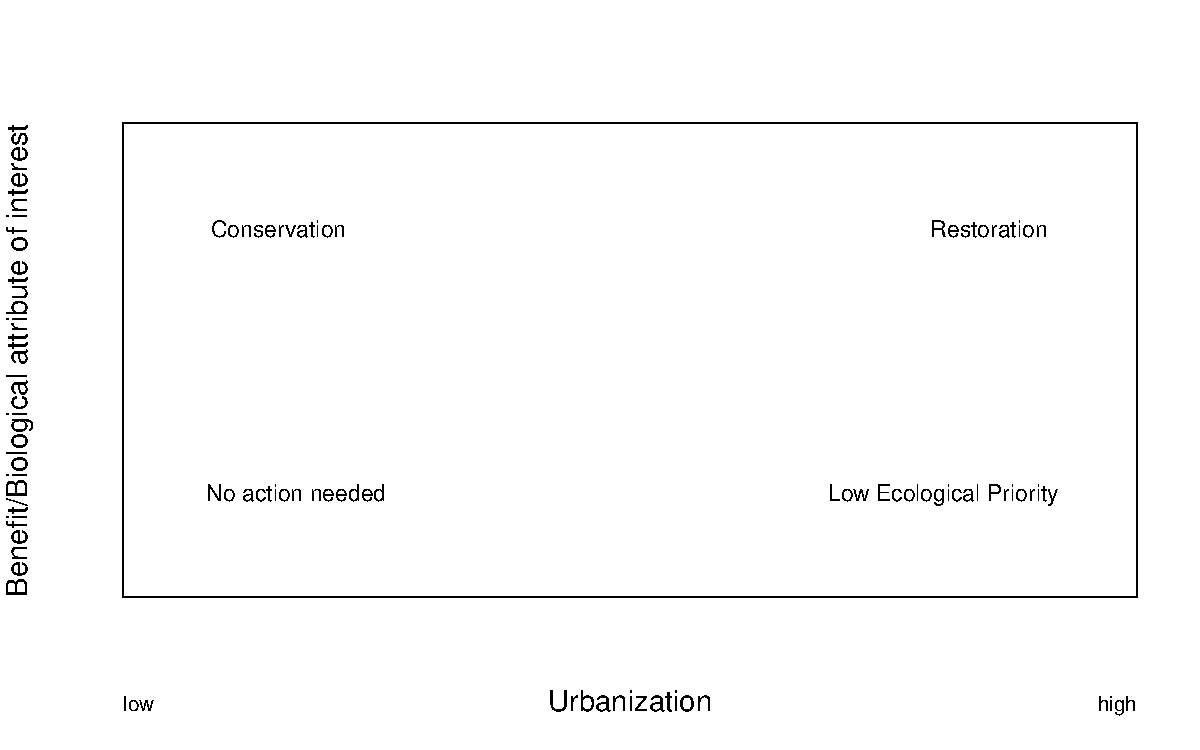
\includegraphics[width=0.75\textwidth]{..//analysis/results/figures/scheme.pdf}
\caption{\textbf{Framework for prioritizing areas of conseration and restoration action} using site-level estimates of coho pre-spawn mortality and urbanization effects.(Need to make this a bit prettier.)}
\label{fig:frame}
\end{figure}

\begin{figure}[h!]
\centering
\noindent 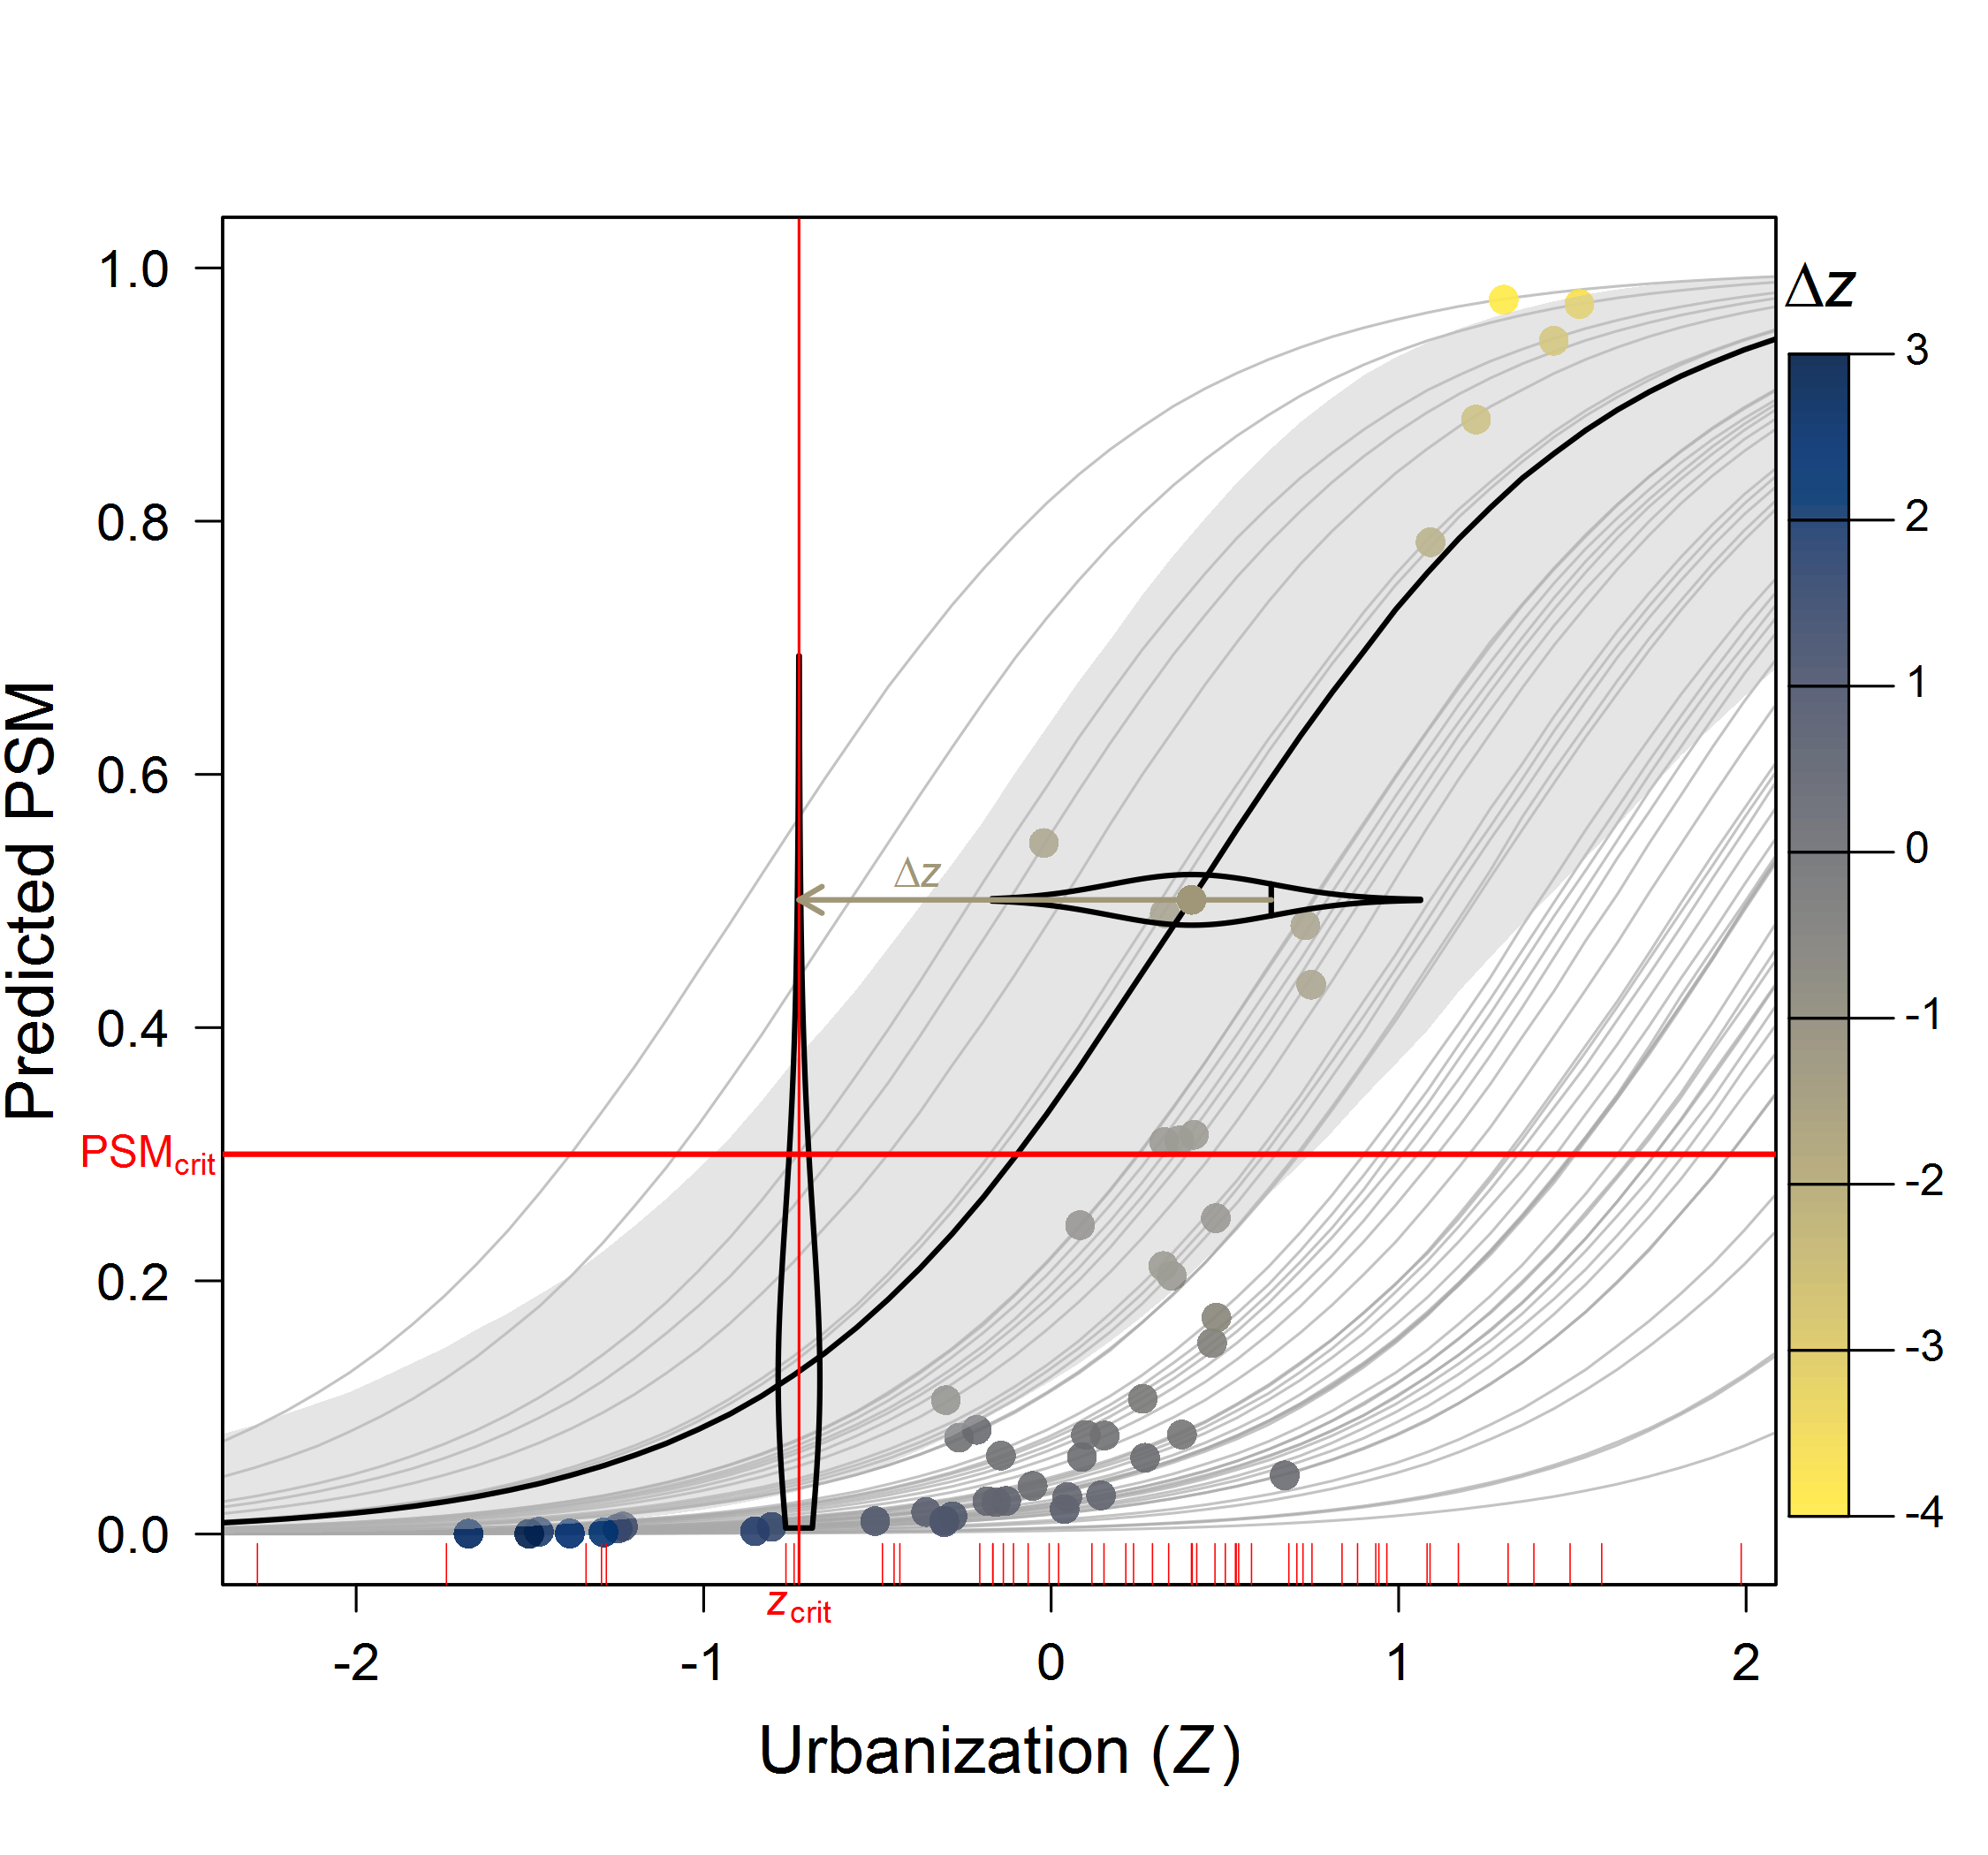
\includegraphics[width=0.75\textwidth]{..//analysis/results/figures/psm_z_threshold.png}
\caption{\textbf{Relationship between estimated pre-spawn mortality and urbanization} based on the structural equation and multi-level modeling in \citep{feist2017}.}
\label{fig:psmz}
\end{figure}

\begin{figure}[h!]
\centering
\noindent 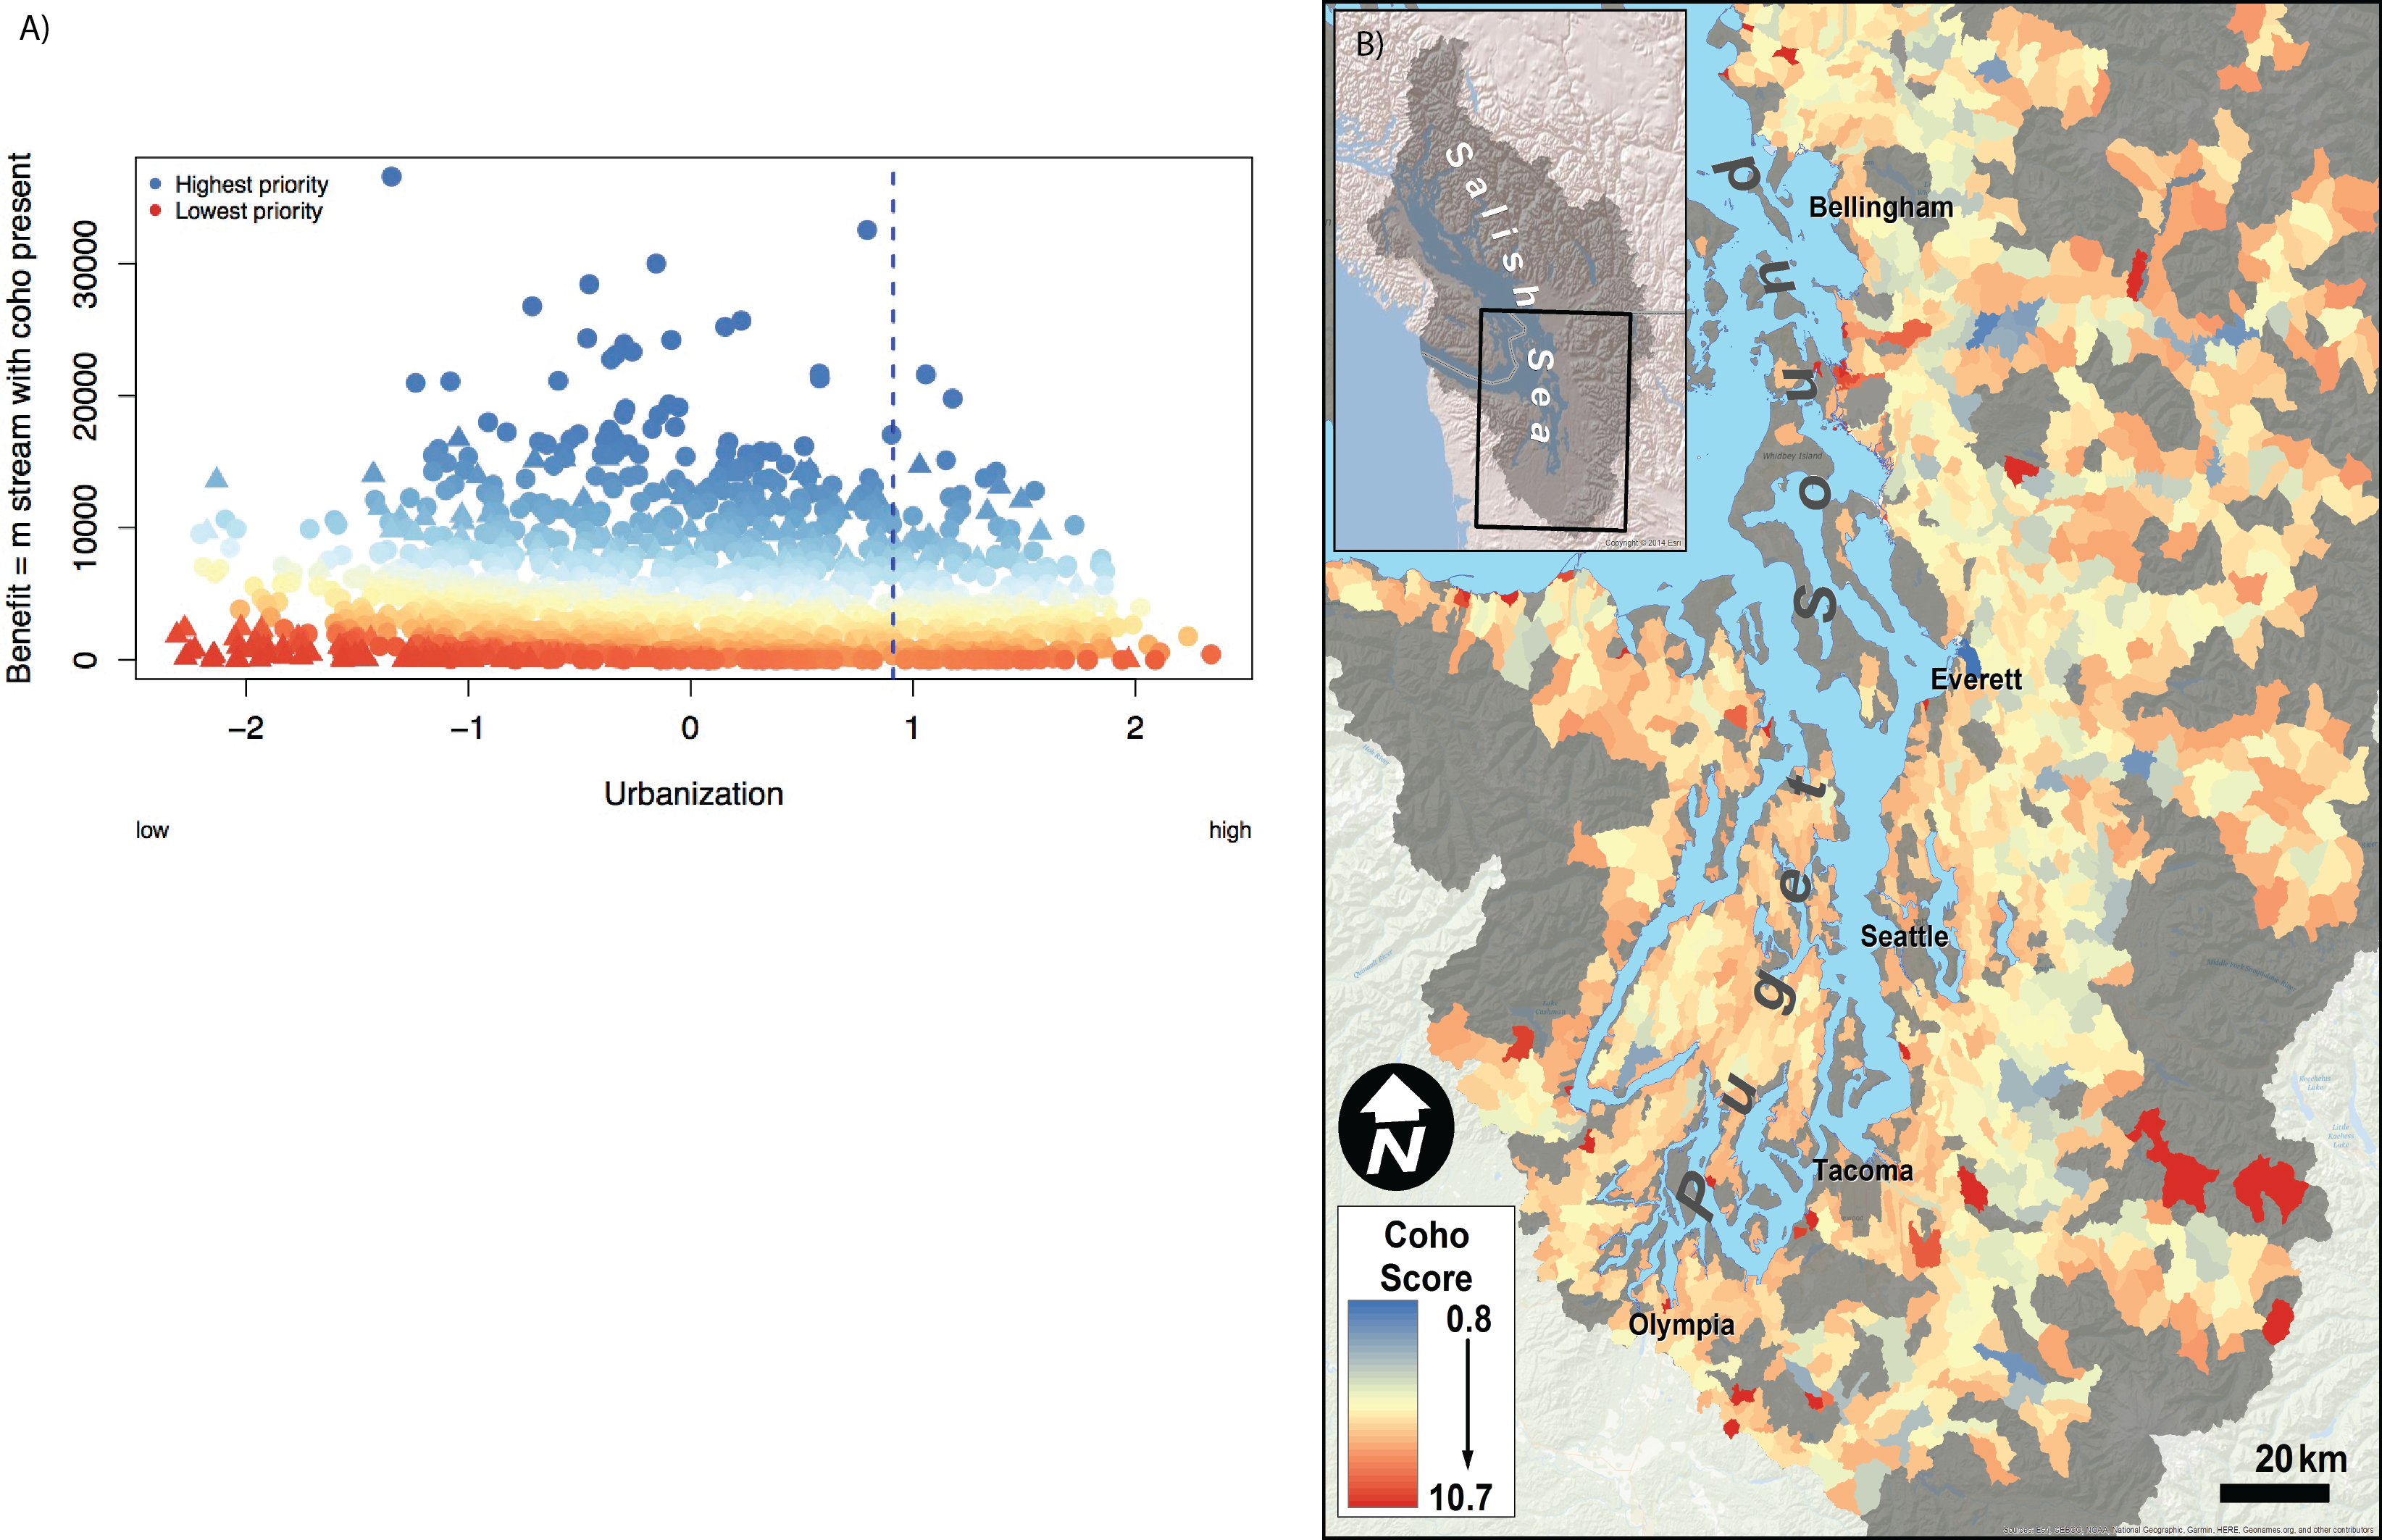
\includegraphics[width=0.75\textwidth]{..//analysis/results/figures/cohopresfig.png}
\caption{\textbf{Prioritization of basins, using meters of stream with coho present} and a critical pre-spawn mortality threshold of 0.25. Lower scores (blue) are higher priority. }
\label{fig:coho}
\end{figure}

\begin{figure}[h!]
\centering
\noindent \includegraphics[width=0.75\textwidth]{..//analysis/results/figures/fallchinfig.png}
\caption{\textbf{Prioritization of basins, using meters of stream with fall chinook present} and a critical pre-spawn mortality threshold of 0.25. Lower scores (blue) are higher priority. }
\label{fig:chin}
\end{figure}

\begin{figure}[h!]
\centering
\noindent 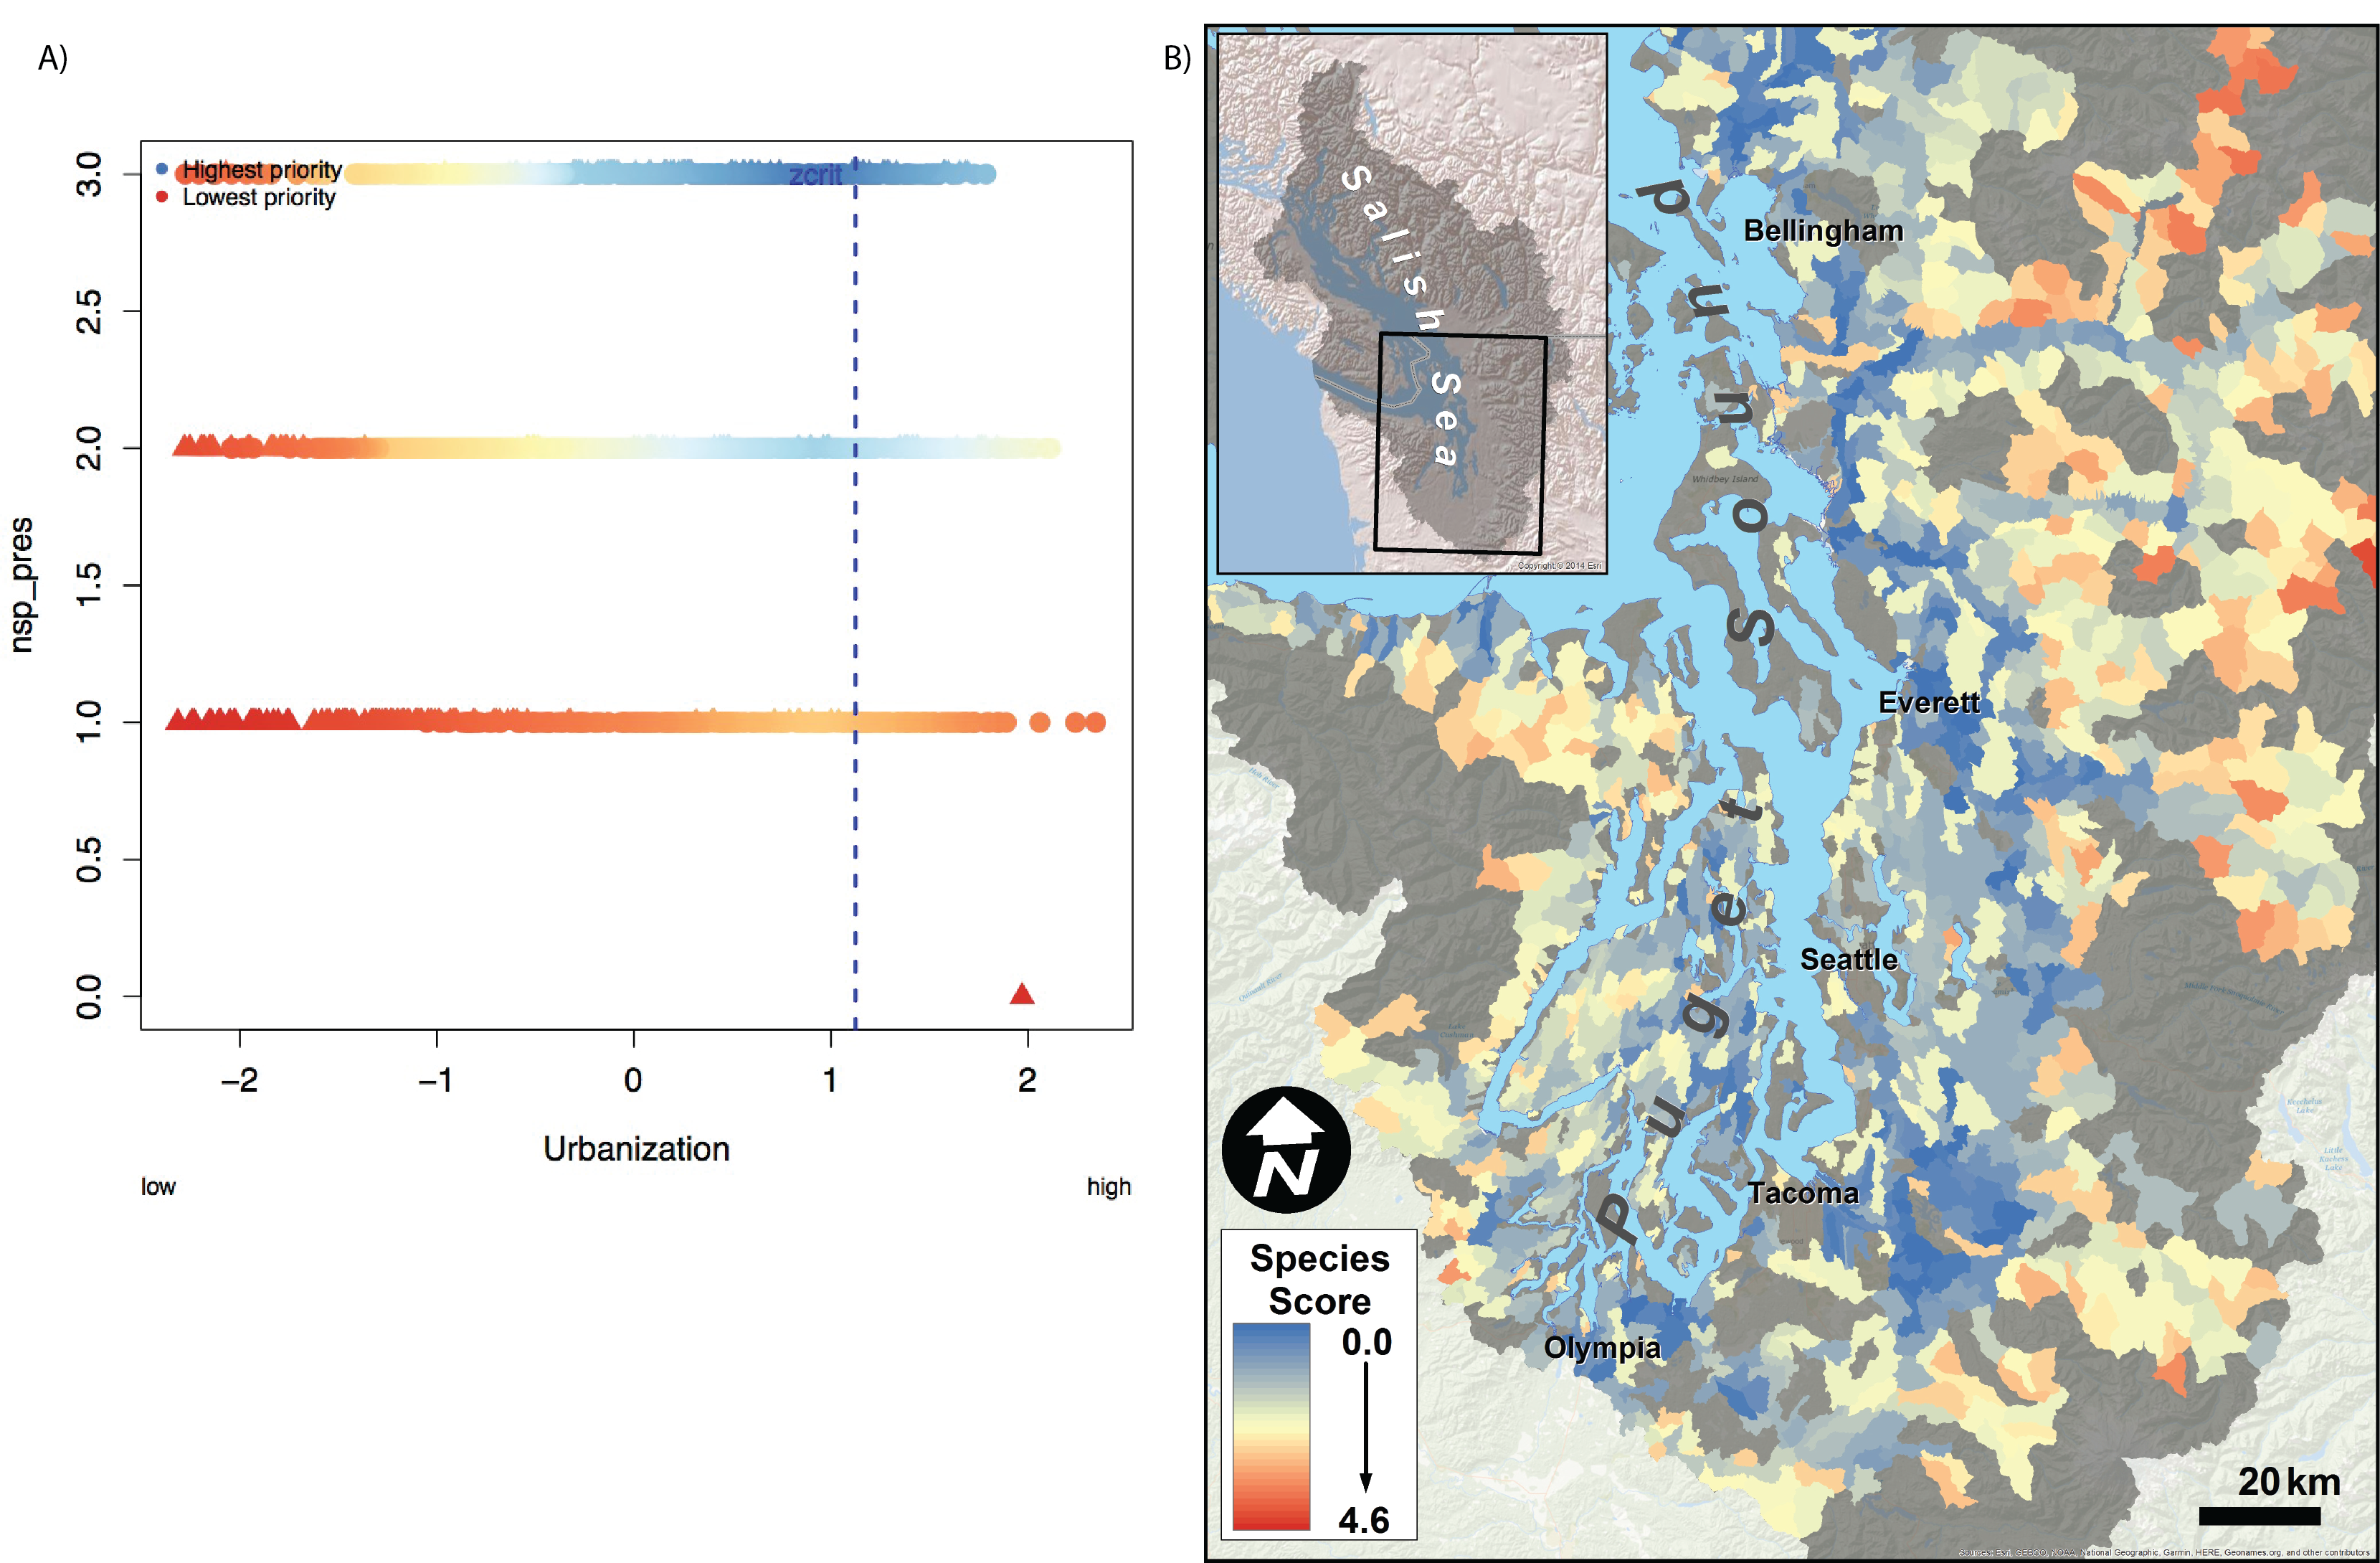
\includegraphics[width=0.75\textwidth]{..//analysis/results/figures/salmsppfig.png}
\caption{\textbf{Prioritization of basins, using the number of salmon species present} and a critical pre-spawn mortality threshold of 0.25. Lower scores (blue) higher priority (and generally have higher numbers of species). }
\label{fig:spp}
\end{figure}
%%%%%%%%%%%%%%%%%%%%%%%%%%%%%%%%%%%%%%%%
\end{document}
%%%%%%%%%%%%%%%%%%%%%%%%%%%%%%%%%%%%%%%%
